\documentclass[10pt,journal]{IEEEtran}

\usepackage[T1]{fontenc}
\usepackage[utf8]{inputenc}
\usepackage{graphicx}
\usepackage{booktabs}
\usepackage{url}
\usepackage[hidelinks]{hyperref}

\graphicspath{{figures/}}

\title{Speech as a Safety Net for Drone Operation}

\author{Zilong Zeng, Junxi Xia, R. Venkatesha Prasad, and Stephen Xia}

\begin{document}

\maketitle

\begin{abstract}
Unmanned Aerial Vehicles (UAVs, or drones) are beginning to operate in shared, low-altitude spaces where nearby people may observe risks before the drone system resolves them on its own. If a drone is drifting toward a wall, moving too close to a person, or continuing a task that should stop, a nearby person should be able to shout an urgent instruction without first reaching a controller, phone application, or networked interface. This article proposes speech as a safety net for drone operation. We describe a drone-side speech-processing path that listens locally, operates in real time, and maps short audio windows into safety-relevant categories: emergency-related speech, movement-related speech, and unsupported input. The resulting category is not treated as an immediate flight command; it is a bounded input that can be kept separate from drone behavior. We outline the design choices behind this framing and summarize implementation evidence from an embedded audio platform, including recognition results, onboard runtime behavior, participant-level live speech trials, and an emergency-related speech demonstration.
\end{abstract}

\begin{IEEEkeywords}
Drone interaction, speech processing, safety net, edge sensing.
\end{IEEEkeywords}

\section{Introduction}
%Drones are beginning to appear in more shared, low-altitude settings rather than only in isolated flight zones. They are increasingly used or proposed for inspection, assistance, education, performance, transportation, parcel delivery, hazardous response, and other tasks near people. In these settings, a drone is not only a remote sensor or flying camera. Its sensing and decisions are tied to a moving physical vehicle that can change the space around it. When drone behavior may affect nearby people, the drone itself, or the surrounding environment, communication becomes part of the safety problem rather than only a matter of convenience. Nearby people therefore need a quick way to express simple or urgent needs, such as asking a drone to move away, hold position, stop a task, or respond to a safety-critical situation, without first finding a controller, opening a mobile phone application, or relying on a networked interface. Spoken input is a natural candidate because voice is immediate, hands-free, and widely treated as a natural modality for human-robot communication~\cite{moore2022vocal}.
Unmanned Aerial Vehicles (UAVs, or drones) are beginning to appear in shared, low-altitude spaces such as classrooms, laboratories, warehouses, inspection sites, and field-support settings. In these environments, a drone may operate autonomously or semi-autonomously while people remain close enough to observe its behavior. Onboard perception, navigation, or task logic may not catch every local risk in time. A nearby person may notice that a drone is drifting toward a wall, approaching a person, or continuing a task that should stop before the drone system resolves the situation on its own. In such moments, human input can become part of the safety picture.

We view the drone in this setting as an embodied computing system: it senses, computes, and acts through a moving physical platform in a space shared with people. A speech safety net therefore supports a boundary for embodied human-drone interaction, where nearby human input may matter before physical consequences occur.

This article proposes speech as a safety net for drone operation. If a drone is about to hit a wall, move too close to a person, or continue a task after the scene has changed, a nearby person should be able to shout ``stop,'' ``move away,'' or ``hold position'' without first finding a controller, opening a mobile phone application, or relying on a networked interface. Speech is a natural candidate for this role because voice is immediate, hands-free, and widely treated as a natural modality for human-robot communication~\cite{moore2022vocal}. The goal is not to replace onboard autonomy or operator control, but to give people in the same space a fast way to express safety-relevant input.

This matters because drone operation has physical consequences. A drone that collides with a wall can damage the vehicle, nearby objects, or the environment; a drone that collides with a person can create injury risk. Regulatory discussions already treat drone operation as a risk-managed activity. Commission Implementing Regulation (EU) 2019/947, for example, frames unmanned aircraft operation around rules and procedures that depend on operating conditions and the protection of people on the ground and other airspace users~\cite{eu2019uasops}. This article argues that, in shared spaces, speech should be considered part of the operating context for safer drone interaction.

We make this idea concrete through drone-side speech processing. Short audio windows are mapped to safety-relevant intent categories: \emph{emergency}, \emph{movement}, and \emph{unknown}. The \emph{emergency} category captures urgent speech that may indicate danger, interruption, or a need to stop. The \emph{movement} category captures ordinary motion-related speech, and \emph{unknown} captures speech or sound that should not be treated as either case.

The article makes three contributions:
\begin{itemize}
    \item It defines speech as a safety-net problem for drone operation in shared low-altitude spaces, where nearby people may observe risks before the drone system resolves them on its own.
    \item It designs a drone-side speech-processing pipeline that maps short audio windows into emergency-related, movement-related, and unsupported categories.
    \item It implements the pipeline on a XIAO ESP32-S3 Sense board and shows that the embedded path can support real-time local audio capture and inference.
\end{itemize}

%However, speech near a drone is not the same as speech to a phone, smart speaker, or cloud assistant. The drone listens from within a changing physical environment: its rotors add noise, its motion changes the distance and angle to the speaker, and nearby people or wind may overlap with the intended utterance. As a result, a phrase may be missed, a background conversation may be treated as relevant, or an urgent stop request may be confused with ordinary movement-related speech. In this setting, a speech error is not only an interface failure. If the error is passed downstream without caution, it may contribute to unsafe behavior, such as a drone continuing a task when someone is trying to interrupt it, moving when it should hold position, or ignoring speech that signals danger to the drone, its surroundings, or nearby people.

%This article argues that spoken interaction with drones needs a safety net between nearby speech and vehicle-facing behavior. The core pipeline is not speech directly becoming action. Instead, nearby audio should first be interpreted by a speech-processing model that can recognize whether the speech is emergency-related, movement-related, or neither. A transcript may be useful in some interfaces, but it is not the required first representation. For drones, the more important step is to turn noisy nearby speech into a compact signal that separates urgent, motion-related, and unsupported speech before it matters to the vehicle.

%We make this safety-net framing concrete through drone-side speech processing. Short audio windows are processed locally and mapped to three categories: \emph{emergency}, \emph{movement}, and \emph{unknown}. The \emph{emergency} category covers urgent speech that may indicate danger, interruption, or a need to stop. The \emph{movement} category covers speech that appears related to ordinary drone motion, such as moving, holding position, or changing direction. The \emph{unknown} category covers speech or sound that should not be treated as either emergency-related or movement-related input. This small vocabulary gives the safety net a practical starting point: urgent speech, ordinary movement-related speech, and input that should not be acted on are kept separate from the beginning.

\section{System Frame}

The safety-net idea becomes clearer when viewed as a small set of design choices rather than as a single recognition model. In this article, the system frame has three choices: the safety net is based on speech, the first processing step runs on the drone side, and the result must be available in real time. These choices are motivated by the same requirement: nearby speech should be usable when a person observes that a drone may be entering a risky situation without depending on an external interface, network path, or delayed interpretation.

The first design choice is to focus on speech as the input to the safety net. A nearby person may shout an interruption, warning, or motion-related request while watching the drone operate. Rotor noise, microphone placement, motion, and distance all shape the audio before any software sees it. A speech-to-text system is useful when the interface needs readable language, for example for logging, display, or later human review. Prior drone speech studies show that transcript-based voice control can be possible, but they also show that rotor noise and platform conditions make word recognition fragile around drones~\cite{oneata19_interspeech,miesikowska2021uavnoise}. We therefore do not use speech-to-text as the default path. In short, noisy, or urgent interaction, recovering every word can be both difficult and unnecessary. For the safety net, the first question is simpler: is the nearby speech emergency-related, movement-related, or unsupported? A direct audio model can answer that question as a compact category, avoiding an extra transcript step before the safety net receives the speech-derived signal. This design is closer to limited-vocabulary speech recognition than to open-ended dictation, where the goal is to recognize a small set of useful speech categories under constrained conditions~\cite{warden2018speechcommands}.

The second design choice is to keep the speech-processing step on the drone side. Spoken interaction around a drone should not assume that a nearby person can open a phone application, pair with a controller, or reach a cloud speech service before communicating. These assumptions are especially weak for emergency-related speech, where the person who needs to speak may be a bystander rather than the trained operator. Local processing also keeps the microphone, rotor noise, and first interpretation in the same physical setting. This requirement aligns with prior work on microcontroller speech and embedded inference, which shows that small-footprint speech models and TinyML runtimes can support local audio decisions under memory and operator constraints~\cite{zhang2017helloedge,david2021tflm,lin2020mcunet,banbury2021mlperftiny}.

The third design choice is real-time speech processing. Speech that indicates a need to stop, move away, or hold position loses value if it is interpreted only after the scene has changed. The speech module should therefore operate at the pace of the interaction: audio is captured in short windows, processed locally, and converted into a safety-net category quickly enough for the drone system to use. This timing requirement is another reason to avoid making full transcription the default first step. The safety net benefits from a compact output that can be produced under rotor-noisy conditions before the speech becomes stale.

Together, these choices define how the safety net should work. The speech module is not expected to make the drone understand arbitrary language. It turns nearby speech into a local, timely, and limited category: emergency-related speech, movement-related speech, or unsupported input. The safety net then keeps that category separate from immediate drone behavior. This gives the drone system a practical starting point while preserving the boundary that speech should not become physical behavior by default.

\section{Implementation and Evaluation}

We implemented drone-side speech processing on a small embedded audio platform. The setup uses a XIAO ESP32-S3 Sense board placed near the drone, with the board microphone capturing nearby speech. Each input is a one-second window of 16~kHz mono audio. The speech processor first converts the waveform into log-mel time-frequency features. A compact neural classifier, with a small convolutional frontend followed by temporal sequence modeling, then processes these features onboard and returns a safety-net category: \emph{emergency}, \emph{movement}, or \emph{unknown}.

The controlled recognition experiments use Google Speech Commands utterances mapped into the three safety-net categories and mixed with locally captured drone rotor audio. The participant study is used only for live onboard evaluation, not for training.

\begin{figure*}[t]
    \centering
    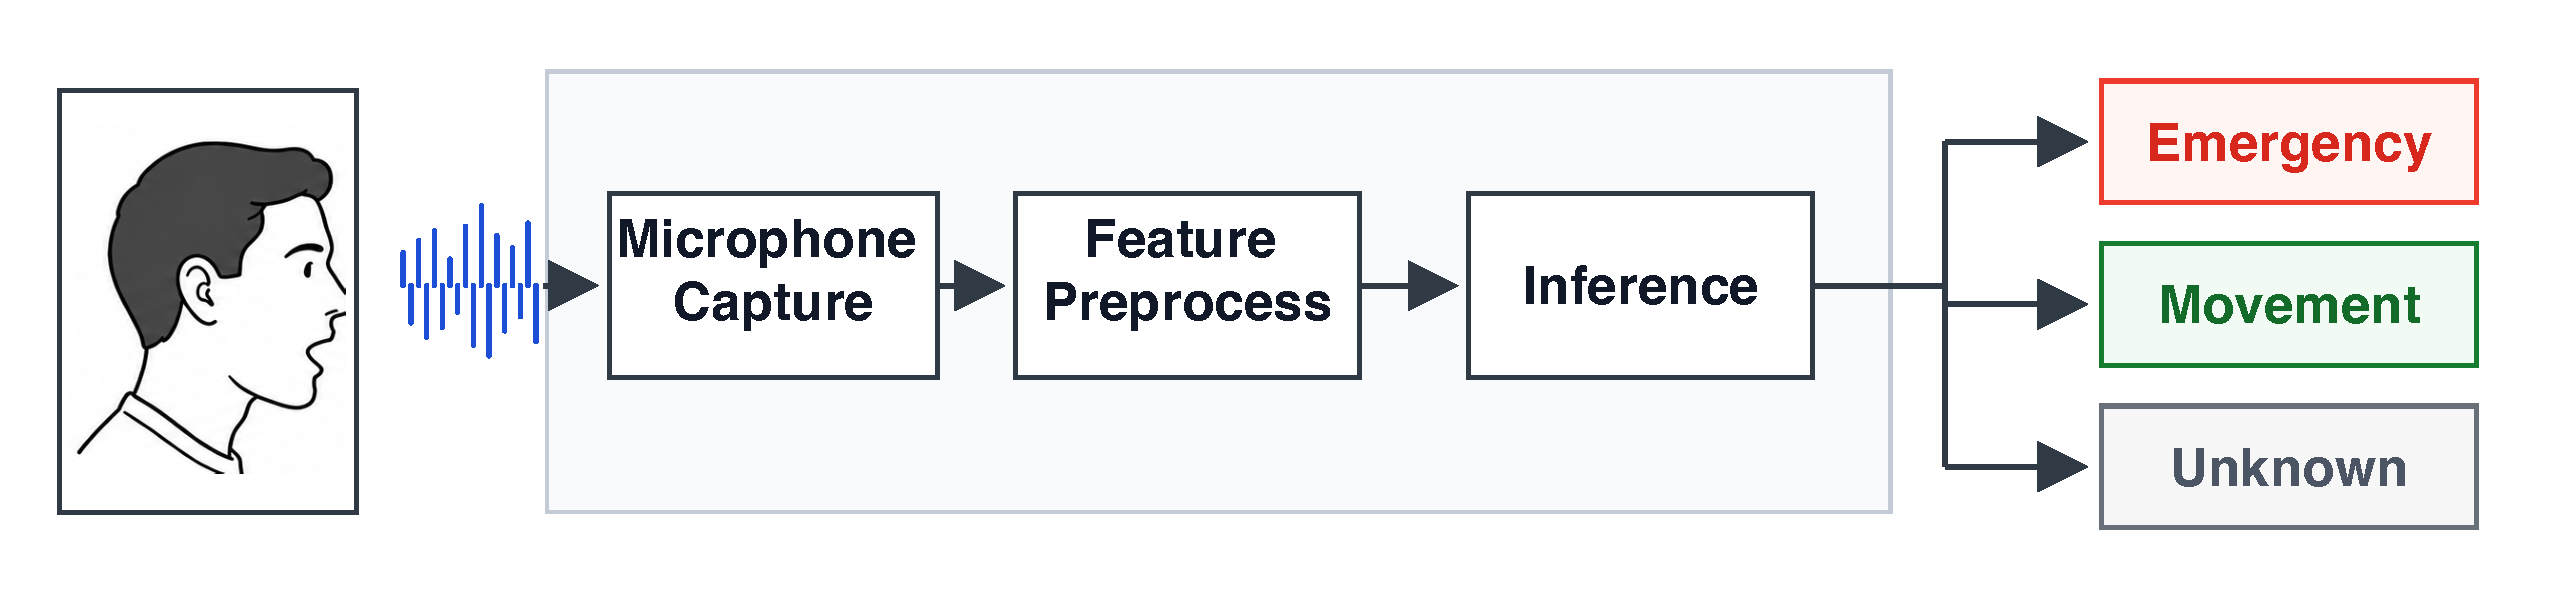
\includegraphics[width=\textwidth]{figures/onboard_speech_pipeline.pdf}
    \caption{Drone-side speech-processing pipeline.}
    \label{fig:onboard_speech_pipeline}
\end{figure*}

Figure~\ref{fig:onboard_speech_pipeline} shows the drone-side pipeline. Nearby speech is captured by the microphone on the XIAO ESP32-S3 Sense board, keeping sensing close to the drone's acoustic condition, including rotor noise, microphone placement, and the changing geometry between the speaker and vehicle. The captured audio is then converted into log-mel features and passed to the onboard classifier for real-time inference. The pipeline ends with one of three safety-net categories: \emph{emergency}, \emph{movement}, or \emph{unknown}. Because this first interpretation runs locally, the interaction does not depend on a phone application, cloud speech service, or reliable network path at the moment when nearby speech is produced.

This implementation is intentionally narrow. It does not attempt to parse open-ended language, estimate a complete dialogue state, or decide how the drone should move. It focuses on the first part of the safety-net path: can the drone-side device listen in the relevant acoustic setting and produce a compact speech-derived signal quickly enough to be useful? 

We summarize four kinds of evaluation evidence. First, we test the speech module under different rotor-noise SNR conditions to show how changes in the acoustic environment affect speech processing. Second, we compare the safety-net speech-processing design with conventional alternatives, including transcript-first and compact command-recognition baselines, to explain why speech-derived safety-net categories are a more suitable first handoff for spoken drone interaction. Third, we report the embedded runtime behavior to show whether the XIAO ESP32-S3 Sense path can sustain local sensing, feature processing, and inference. Fourth, we report participant-level live speech trials to expose how the onboard path varies across speakers.

\begin{table}[t]
    \centering
    \caption{Speech-processing output under different rotor-noise SNR conditions.}
    \label{tab:snr_results}
    \footnotesize
    \setlength{\tabcolsep}{3pt}
    \begin{tabular}{@{}lcc@{}}
        \toprule
        SNR & Acc. & Emerg. recall \\
        \midrule
        -10~dB & 0.86 & 0.86 \\
        -15~dB & 0.83 & 0.85 \\
        -20~dB & 0.76 & 0.81 \\
        \bottomrule
    \end{tabular}
\end{table}

Table~\ref{tab:snr_results} shows how the speech module changes as rotor noise becomes stronger. Accuracy decreases as the SNR moves from -10~dB to -20~dB, while emergency recall remains at or above 0.81 across the tested conditions. This trend is important for the article's framing: spoken drone interaction is shaped by the acoustic environment, so the safety net should begin with a speech-derived category that is explicit about what the audio system can and cannot separate under noise.

\begin{table}[t]
    \centering
    \caption{Comparison with transcript-first and compact command-recognition baselines on rotor-noisy one-second clips at -10~dB SNR.}
    \label{tab:baseline_comparison}
    \footnotesize
    \setlength{\tabcolsep}{3pt}
    \begin{tabular}{@{}p{0.48\linewidth}cc@{}}
        \toprule
        Method & Acc. & Emerg. recall \\
        \midrule
        Drone-side speech processor & 0.86 & 0.86 \\
        Whisper \texttt{tiny.en} + parser & 0.43 & 0.22 \\
        DS-CNN-S family & 0.61 & 0.78 \\
        \bottomrule
    \end{tabular}
\end{table}

Table~\ref{tab:baseline_comparison} explains why the system is framed around speech processing for a safety net rather than raw transcripts or ordinary command recognition at the -10~dB comparison point. The transcript-first pipeline performs poorly on the short noisy windows because it must first recover usable text before the safety-net category can be inferred. The compact command-recognition baseline is closer to the proposed path, but it still treats the audio problem as ordinary label selection. The drone-side speech processor instead makes the output match the interaction need: separating emergency speech, movement-related speech, and unsupported input before later drone-facing decisions are considered.

The embedded runtime result checks whether this pipeline can run locally. In a dual-core onboard timing run over 120 one-second windows, more than 95\% of clips were processed at approximately the one-second window rate after the first update, with no dropped or overrun windows.

We also collected live speech from 11 participants using the same onboard capture-to-inference path. The study included prompted utterances across the three safety-net categories and produced 1462 total samples. Table~\ref{tab:participant_live_trials} reports participant-level emergency recall and overall accuracy. The lower emergency recall in these live trials should be read together with the controlled SNR results. The SNR tests use fixed one-second clips under controlled mixtures, while the participant trials introduce live speech variation, including speaking rate, pronunciation, delivery, microphone alignment, and collection-condition mismatch. The relatively large standard deviation therefore highlights cross-speaker variability, which motivates the cross-user robustness work discussed in Section~V.


\begin{figure*}[t]
    \centering
    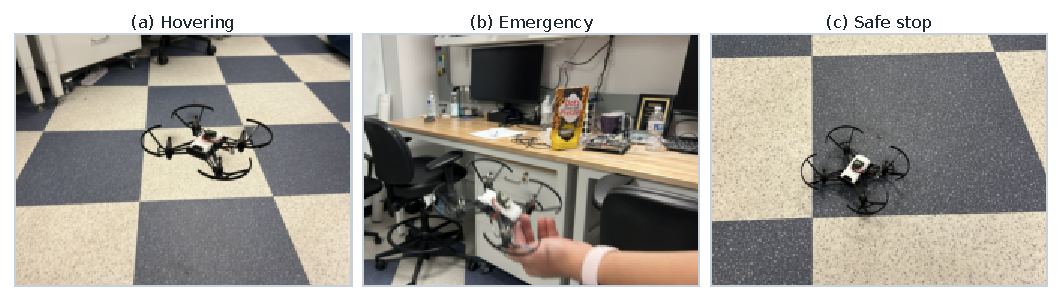
\includegraphics[width=\textwidth]{figures/emergency_stop_sequence.pdf}
    \caption{Emergency-related speech demonstration scene. A nearby person speaks toward the drone, the onboard pipeline continues processing local audio, and the system presents the detected emergency-related speech as the relevant safety-net signal for the scene.}
    \label{fig:emergency_demo}
\end{figure*}

Figure~\ref{fig:emergency_demo} shows the setting behind the emergency case. A person near the drone produces urgent speech, the drone-side audio pipeline processes the input locally, and the output is treated as emergency-related speech rather than as an open-ended transcript or ordinary movement command. This scene shows how the safety-net framing appears in a concrete spoken-drone interaction.

\begin{table}[t]
    \centering
    \caption{Participant-level user study using onboard capture and inference.}
    \label{tab:participant_live_trials}
    \footnotesize
    \setlength{\tabcolsep}{4pt}
    \begin{tabular}{@{}lccc@{}}
        \toprule
        Speakers & Number of Samples & Emerg. recall & Acc. \\
        \midrule
        11 & 1462 & 0.623 $\pm$ 0.148 & 0.764 $\pm$ 0.079 \\
        \bottomrule
    \end{tabular}
\end{table}

\section{Real-World Applications and Vision}

The preceding sections describe why spoken drone interaction needs a safety net and how drone-side speech processing can support it. The broader question is where this framing matters in practice. Prior work has explored speech interaction for drones in settings such as automatic speech recognition, multimodal recognition, and voice-driven drone control~\cite{oneata19_interspeech,oneata2021multimodal,park2023uavvehicle}. Our focus is narrower: shared, low-altitude spaces where drones operate near people who may need to interrupt, redirect, or call attention to the vehicle quickly.

One example is education and research. Small drones are increasingly used in labs and classrooms for demonstrations, programming exercises, and robotics instruction. In these settings, the person who notices a problem may be a student or observer rather than the instructor holding the controller. A spoken safety net could make urgent speech, such as a request to stop or hold position, visible to the system without assuming that every student knows the exact command interface.

Another example is inspection and logistics. In warehouses, construction sites, and infrastructure inspection tasks, workers may have occupied hands, protective equipment, or limited access to a phone. The drone may be close enough for speech to be natural but not close enough for direct physical intervention. Here, the value of the safety net is not that speech replaces the operator. It is that safety-relevant speech can be separated from ordinary workplace noise and made available before it is treated as drone behavior.

Hazardous-response and field-support settings add a different pressure. A person near the drone may need to communicate while moving, carrying equipment, or reacting to a changing scene. Network connectivity may be unreliable, and the person speaking may not be the one who configured the drone. In such cases, relying on a cloud assistant or phone-mediated interface is a weak assumption. A drone-side speech path gives the system a local way to hear urgent nearby speech even when other interfaces are delayed or unavailable.

These applications also make the audio problem more difficult. Drones operate inside the acoustic environment they create. Rotor noise, wind, payload vibration, distance, and changing orientation all affect what the microphone hears. Drone-audition research identifies ego-noise, payload limits, and onboard processing as recurring constraints for aerial audio systems~\cite{chevtchenko2025drone_ssl}. A speech safety net therefore has to be designed for the drone's local sensing condition, not only for clean speech recorded near a stationary device.

The long-term vision is a safety net that supports nearby speech without turning speech into open-ended command authority. Emergency-related speech should remain visible as a safety-relevant signal. Movement-related speech should remain distinguishable from urgent interruption. Unsupported input should not be forced into drone-relevant meaning. Future systems can connect these outputs to operator awareness, confirmation, context-aware safety rules, or multimodal sensing. For example, a classroom system might surface a student's urgent stop request to the instructor interface; a warehouse system might separate a worker's emergency call from aisle noise; a field system might preserve local speech-derived alerts when a phone interface or network path is unreliable.

This vision keeps the article's role modest. The safety net is not a complete drone safety architecture, and speech processing is not a substitute for existing safeguards. Instead, spoken input becomes one local, timely source of information that can be handled before any later drone-facing decision. That framing is what makes voice useful for shared-space drone interaction without treating every nearby utterance as a command.

\section{Limitations and Future Work}

This article presents a safety-net framing for spoken drone interaction in shared physical spaces. We argue that nearby speech should be processed on the drone side and in real time before it can matter to drone behavior. We develop three design choices for this framing: focusing on speech as the safety-net input, keeping the first speech-processing step local to the drone, and producing timely categories for emergency-related speech, movement-related speech, and unsupported input. We then describe an implementation on a XIAO ESP32-S3 Sense board and summarize evidence from rotor-noisy speech processing, baseline comparison, embedded runtime, and an emergency-related speech scene.

The first limitation is the small category space. The current safety net uses \emph{emergency}, \emph{movement}, and \emph{unknown} because these categories make the main interaction boundary easy to explain: urgent speech, ordinary motion-related speech, and input that should not be acted on are kept separate. Real deployments may need more categories, such as hold, land, return, resume, cancel, request attention, or ask for help. Expanding the vocabulary should be done carefully. Each new category should correspond to a clear interaction need near the drone, not merely to a larger command list.

A related direction is to extend simple speech processing toward stronger intent analysis and recognition. Prior spoken-language-understanding work shows that systems can move from audio toward semantic or intent decisions without relying only on full transcripts~\cite{haghani2018audio_semantics,lugosch19_interspeech,kuo20_interspeech,le2022deliberation}. This direction is useful because different utterances can express the same underlying need. For example, ``stop,'' ``wait,'' and ``do not move closer'' may all indicate an interruption or safety-related request. Similar drone-relevant intent may also appear across languages, accents, and speaker groups, even when the surface words differ. Future systems could therefore learn language- or user-specific expressions while preserving a shared set of drone-relevant intents. This would let the safety net support more diverse speakers without assuming that everyone uses the same words.

Cross-user and cross-language robustness should be studied together with the acoustic setting. Emergency speech may be shouted, repeated, clipped, or masked by rotor noise. A visitor, child, worker, or first responder may use different vocabulary and different levels of urgency. Future datasets should therefore include more speakers, languages, environments, microphone placements, and drone operating conditions. The goal is not only higher recognition accuracy, but a clearer understanding of when the speech-processing module should produce an actionable category and when it should remain conservative.

The implementation can also be improved. On-device speech processing must balance latency, memory, energy, microphone placement, and model size. Future implementations may use better audio front ends, adaptive noise handling, model compression, or hardware-aware scheduling to make the pipeline more reliable across drone platforms. These optimizations matter because the safety-net idea depends on speech being available locally and quickly, especially when a phone or cloud service is unavailable.

Finally, speech should eventually be combined with context and other sensing modalities. Speech alone may be ambiguous when the speaker is far away, not addressing the drone, or masked by noise. Visual cues, gesture, localization, flight state, proximity to people, and task context can help decide whether nearby speech is relevant and how conservatively the drone system should respond.


\bibliographystyle{IEEEtran}
\bibliography{references}

\end{document}
